\section{PkID中用到的特征}
PkID中用到的特征一共有67个:Area, Mean, StdDev, Mode, Min, Max, X, Y, XM, YM, Perim., BX, BY, Width, Height, Major, Minor, Angle, Circ., Feret, IntDen, Median, Skew, Kurt, \%Area, XStart, YStart, Area\_exc, Fractal, Skelarea, Slope, Histcum1, Histcum2, Histcum3, XMg5, YMg5, Compentropy, Compmean, Compslope, CompM1, CompM2, CompM3, Symetrieh, Symetriev,Tag, ESD, Elongation, Range, MeanPos, CentroidsD, CV, SR, PerimAreaexc, FeretAreaexc, PerimFeret, PerimMaj, Circexc, CDexc, {\color{blue}Nb1, Nb2, Nb3,  Symetriehc, Symetrievc, Convperim, Convarea, Fcons, ThickR(这几个特征没有找到具体的含义)}

从训练集的PID文件文件中看到,Compentropy, Compmean, Compslope, CompM1, CompM2, CompM3这6个特征在所有图像上的值都为0,Tag这个特征在所有图像上的值都为1,在训练分类器时是不起作用的,同时这7个特征的具体含义也没有找到。

\subsection{位置特征}
\begin{description}
\item[BX] 能够包围物体,且平行于图像两条边的最小外界矩形的左上角顶点的X坐标 
\item[BY] 能够包围物体,且平行于图像两条边的最小外界矩形的左上角顶点的Y坐标 
\item[Height] 能够包围物体,且平行于图像两条边的最小外界矩形的高
\item[Width] 能够包围物体,且平行于图像两条边的最小外界矩形的宽
\item[XStart] 图像最左上角像素点的X坐标
\item[YStart] 图像最左上角像素点的Y坐标
\item[XM] 物体灰度重心的X坐标
\item[YM] 物体灰度重心的Y坐标
\item[XMg5] gamma值为51时的物体灰度重心的X坐标(gamma值表示图像输出值与输入值关系的斜率)
\item[YMg5] gamma值为51时的物体灰度重心的Y坐标
\item[X] 物体重心点的X坐标
\item[Y] 物体重心点的Y坐标
\item[Angle] 浮游动物主轴与图片x轴形成的夹角,在图片切割后旋转图片测量相关参数使用
\end{description}

这类特征反映的是浮游动物在图像中的位置信息,浮游动物特征与位置信息无关,因此它们不适合作为特征直接用于分类(会降低分类的准确率),而是用来计算其他特征(尺寸特征、灰度特征和形状特征)。

\subsection{尺寸特征}

\begin{description}
\item[Area] 物体的表面积,方形像素的个数%包含物体的最小矩形面积 
\item[Perim] 周长,物体最外层边缘的长度
\item[Major] 物体的最佳拟合椭圆的长轴%物体内切椭圆的长轴
\item[Minor] 物体的最佳拟合椭圆的短轴%物体内切椭圆的短轴
\item[Feret] Maximum feret diameter(最大费雷特径), 沿物体边缘任意两个点的最长距离
\item[Area\_exc] 去掉物体空洞后的表面积,空洞是指灰度值与背景相同的部分
\item[\%area] 物体表面积中空洞所占的百分比,即背景所占的比例
\end{description}

这类特征表示了图像中目标的大小尺寸。它的根据是同类浮游动物的表面积、周长等尺寸特征应该是大致相同的。但是这些特征还存在着问题:1、同类浮游动物在不同时期(如幼年和成年)的个体大小尺寸是不同的。2、拍摄照片的方位不同(比如正面和侧面)得到的尺寸特征也是不同的。

\subsection{灰度值特征}

\begin{description}
    \item[Min] 物体内部所有像素点的最小灰度值 (0 = black)
    \item[Max] 物体内部所有像素点的最大灰度值 (255 = white)
    \item[IntDen (Integrated density)] 总密度,物体内像素点的灰度值的总和($IntDen = Area * Mean$)
    \item[Slope] 归一化的灰度累计直方图的斜率
    \item[Histcum1] 灰度累计直方图的值为25\%时所对应的灰度值
    \item[Histcum2] 灰度累计直方图的值为50\%时所对应的灰度值
    \item[Histcum3] 灰度累计直方图的值为75\%时所对应的灰度值
    \item[CentroidsD] $\sqrt{(XM-X)^{2}+(YM-Y)^{2}}$ 目标物体重心和灰度重心之间的距离。
\end{description}

%这类特征描述的是浮游动物的灰度特征,其中Min、Max、StdDev、Range反映了图像中目标的灰度范围,Skew、Kurt、Slope、Histcum1、Histcum2、Histcum3、Mean、IntDen、Mode、Mean\_exc、Median反映了目标整体的灰度变化和集中趋势,CentroidsD、CV、SR还不清楚它们的物理意义。

根据是同类浮游动物的灰度特征(灰度的范围和整体灰度变换趋势)应该是相似的,但观察图像发现并不是所有同类浮游动物的灰度都是相似的,例如Gelatinous类中有的个体灰度跨度较小,整体灰度都较浅,而有的个体灰度跨度较大;同时由于拍摄时光线的原因,会造成同类浮游动物中个体灰度的深浅不一。

\subsection{形状特征}

\begin{description}
    \item[Fractal] 物体边界的分形维数 (Berube and Jebrak, 1999),表明物体边界的不规则程度
    \item[Skelarea] 骨架像素的表面积(在二值图像中,不断地从物体边缘处减去像素点直到仅剩一个像素的宽度,最后所得图形的像素点数)
    \item[Symetrieh] 水平对称
    \item[Symetriev] 垂直对称
    \item[Circ] $Circularity = (4 * Pi * Area) / Perim^2$ 圆形度,表征物体接近圆的程度,值等于1时,说明物体为正圆形,值越接近0,物体体形越长。
    \item[ESD] $2 \times \sqrt{\cfrac{Area}{\pi}}$ 相应球形直径(也称为等效球直径),是指一不规则外形物体,其体积相同球体的直径。
    \item[Elongation] $\cfrac{Major}{Minor}$ 延伸率,最佳拟合椭圆的长轴和短轴之比。
    \item[Circexc] $\cfrac{4 \times \pi Area\_exc}{Perim^{2}}$ 去掉目标内部空洞的圆形度。
\end{description}

这类特征描述的是浮游动物的灰度特征,根据的是不同种类浮游动物的形状不同。存在的问题是有不同种类的浮游动物形状相似,例如Appendicularia和Chaetognatha,Bubble和Egg;也有同种浮游动物形状不同,例如Decapoda、Gelatinous。

\subsection{生物统计特征}

\begin{description}
    \item[Mean] 物体内的平均灰度值;物体中所有像素点的灰度值的总和除以总的像素个数    
    \item[Range] $Max-Min$ 极差,灰度的范围。    
    \item[CV] $100 \times \cfrac{StdDev}{Mean}$ 变异系数(也称离散系数或相对偏差),是灰度标准偏差与平均值之比,用百分数表示。
    \item[SR] $100 \times \cfrac{StdDev}{Max-Min}$ 灰度标准差比上极差。
    \item[Skew] 灰度直方图的偏度,衡量灰度分布的不对称性。偏度为负就意味着在概率密度函数左侧的尾部比右侧的长,绝大多数的值位于平均值的右侧。偏度为正就意味着在概率密度函数右侧的尾部比左侧的长,绝大多数的值位于平均值的左侧。偏度为零就表示数值相对均匀地分布在平均值的两侧,但不一定意味着其为对称分布。
    \item[Kurt] 峰度,描述灰度直方图的陡缓程度。 
    \item[Mean\_exc] 物体内部去掉空洞后的平均灰度值 ($Mean\_exc = IntDen / Area\_exc$)
    \item[Median] 物体内像素的灰度值的中值
    \item[StdDev] 物体内像素的灰度值的标准差
    \item[Mode] Modal grey value within the object(可能表示灰度的众数)
\end{description}

\subsection{还没有查找到的特征}
\begin{description}
    \item[MeanPos] $\cfrac{Mean-Max}{Max-Min}$
    \item[PerimAreaexc] $\cfrac{Perim}{\sqrt{Area\_exc}}$ 
    \item[FeretAreaexc] $\cfrac{Feret}{\sqrt{Area\_exc}}$
    \item[PerimFeret] $\cfrac{Perim}{Feret}$
    \item[PerimMaj] $\cfrac{Perim}{Major}$
    \item[CDexc] $\cfrac{\sqrt{(XM-X)^{2}+(YM-Y)^{2}}}{{\sqrt{Area\_exc}}}$ 
\end{description}

\subsection{其他特征}
这些特征并没有在PkID中使用,而是在作者的一个幻灯片中提到的新特征。
\begin{description}
\item[Texture Contrast] 
\item[Cumulation Histogram]
\item[Convex Area]
\item[Symmetry]
\item[Thickness Ratio]
\end{description}


\subsection{实验}

采用以上67个特征,并用随机森林分类器进行训练和分类得到的混淆矩阵如图~\ref{fig: PkID-RF-2-folds-5-repetitions}

\begin{figure}[!ht]
\centering
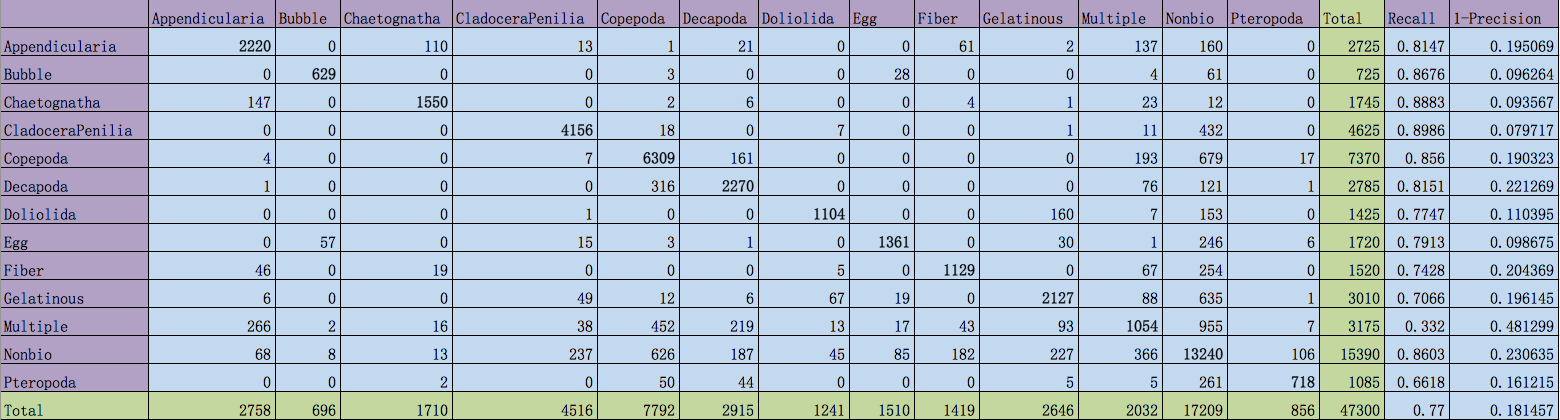
\includegraphics[width=1.0\linewidth]{PkID-RF-2-folds-5-repetitions}
\caption{PkID-RF交叉验证,folds取2,repetitions取5}
\label{fig: PkID-RF-2-folds-5-repetitions}
\end{figure}




